\documentclass[tikz]{standalone}

\usetikzlibrary{arrows, shapes, positioning}

\begin{document}
    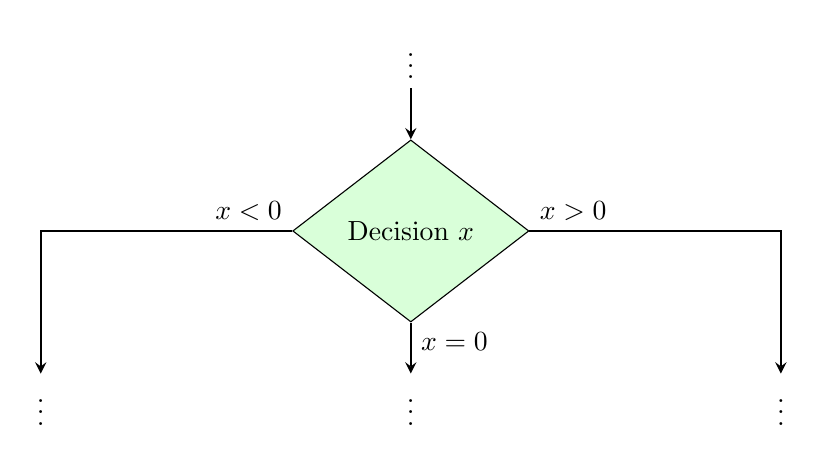
\begin{tikzpicture}[scale=1, node distance=1.7cm]
        \tikzstyle{startstop} = [
    rectangle,
    rounded corners,
    minimum width=3cm,
    minimum height=1cm,
    text centered,
    draw=black,
    fill=red!15
]
\tikzstyle{io} = [
    trapezium,
    trapezium left angle=70,
    trapezium right angle=110,
    minimum width=3cm,
    minimum height=1cm,
    text centered,
    trapezium stretches=true,
    draw=black,
    fill=blue!15
]
\tikzstyle{process} = [
    rectangle,
    minimum width=3cm,
    minimum height=1cm,
    text centered,
    draw=black,
    fill=orange!15
]
\tikzstyle{decision} = [
    diamond,
    minimum width=3cm,
    minimum height=1cm,
    text centered,
    draw=black,
    fill=green!15
]
\tikzstyle{arrow} = [thick, ->, >=stealth]


        \node[] (input) {$\vdots$};
        \node[decision, below of=input,  yshift=-0.5cm] (dec1) {Decision $x$};

        \node[below of=dec1, yshift=-0.5cm] (proc2) {$\vdots$};
        \node[left of=proc2, xshift=-3cm] (proc1) {$\vdots$};
        \node[right of=proc2, xshift=3cm] (proc3) {$\vdots$};

        \draw[arrow] (input) -- (dec1);
        \draw[arrow] (dec1.west) node[above left] {$x<0$} -| (proc1);
        \draw[arrow] (dec1.east) node[above right] {$x>0$} -| (proc3);
        \draw[arrow] (dec1.south) node[below right] {$x=0$} -- (proc2);
    \end{tikzpicture}
\end{document}
